%\mychapter{6}{Results}

\section{Results}
In this section, we report results on  synthetic data using diffusion maps with the $l_{1}$ distance. We compare our results with those obtained via PCA, a popular linear dimensionality technique. We apply PCA and diffusion maps to both the 
clean firing rate data set and the spike time data set preprocessed  with the previous time measure to obtain previous time data.


Figure \ref{fig:DiffMaps_PCA_on_Prevtime_FR} (left column) shows that both diffusion maps with $l_1$  distance and PCA capture the animal's motion around the circular track when applied on firing rate data. This is not surprising since we are using clean firing rate data that encodes the animal's position around the track. However, when using previous time data, diffusion maps with $l_{1}$ distance appears to outperform PCA (see the right column of Figure  \ref{fig:DiffMaps_PCA_on_Prevtime_FR}). We  see that analyzing previous time data using diffusion maps captures the simulated four and half laps taken by the animal around the circular track while PCA  fails to reveal that the rat took four and a half laps  around the track. 

\begin{figure}[H]
        \centering
        \begin{subfigure}[b]{0.475\textwidth}
            \centering
            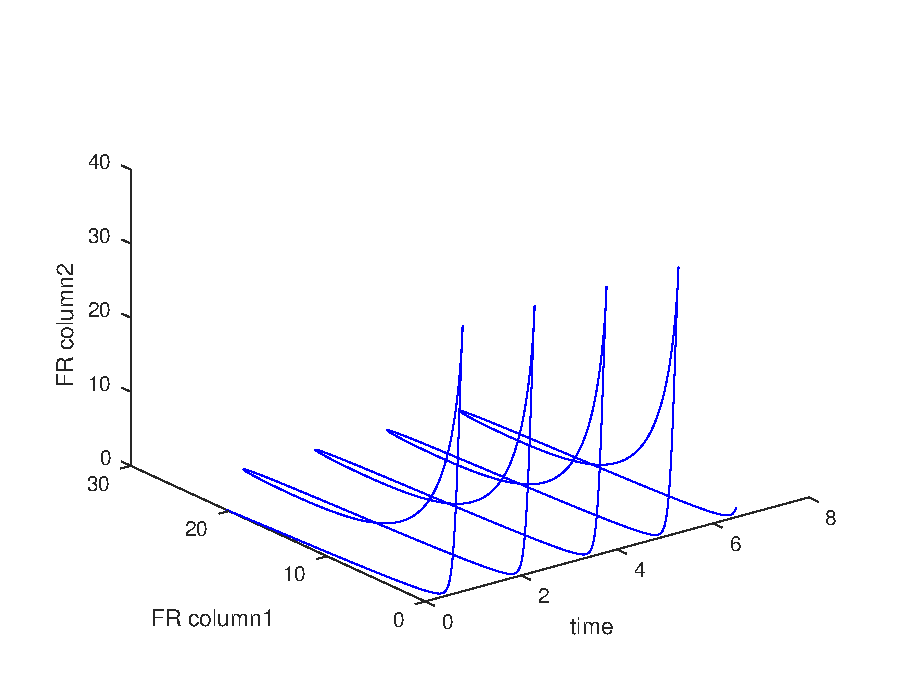
\includegraphics[width=\textwidth]{./images/FinalOralPlots/SyntheticOralPaper/SimFiringRate-with-Time.eps}
           % 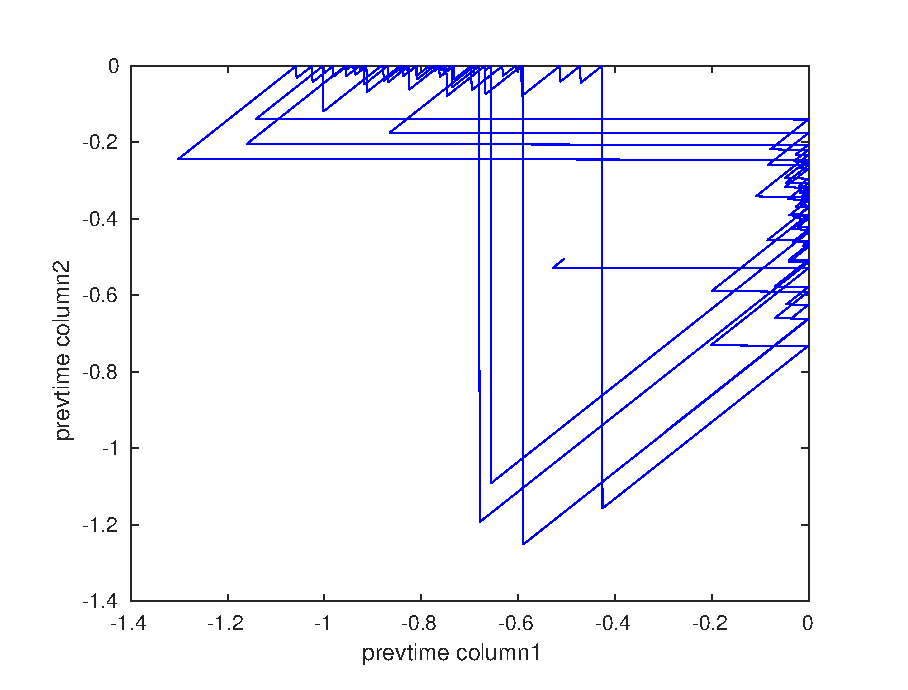
\includegraphics[width=\textwidth]{./images/FinalOralPlots/SyntheticOralPaper/SimPrevtime.eps}
            \caption[]%
            {{\small Simulated firing rate data (FR)}}  
            %{{\small Simulated previous time data (Prevtime)}} 
               
            \label{fig:Prevtime in 3D}
        \end{subfigure}
        \hfill
        \begin{subfigure}[b]{0.475\textwidth}  
            \centering 
           % 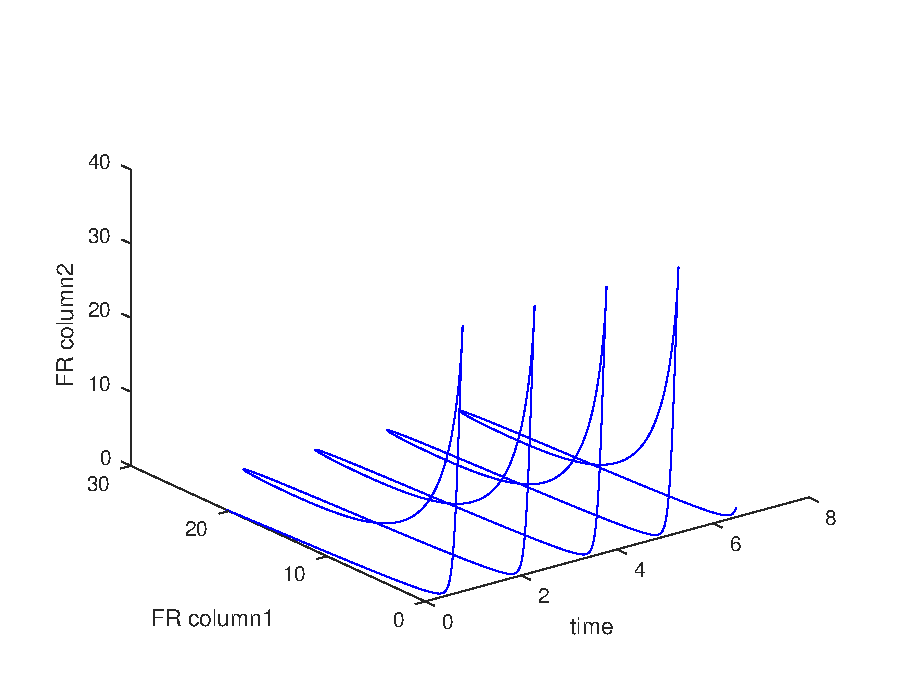
\includegraphics[width=\textwidth]{./images/FinalOralPlots/SyntheticOralPaper/SimFiringRate-with-Time.eps}
            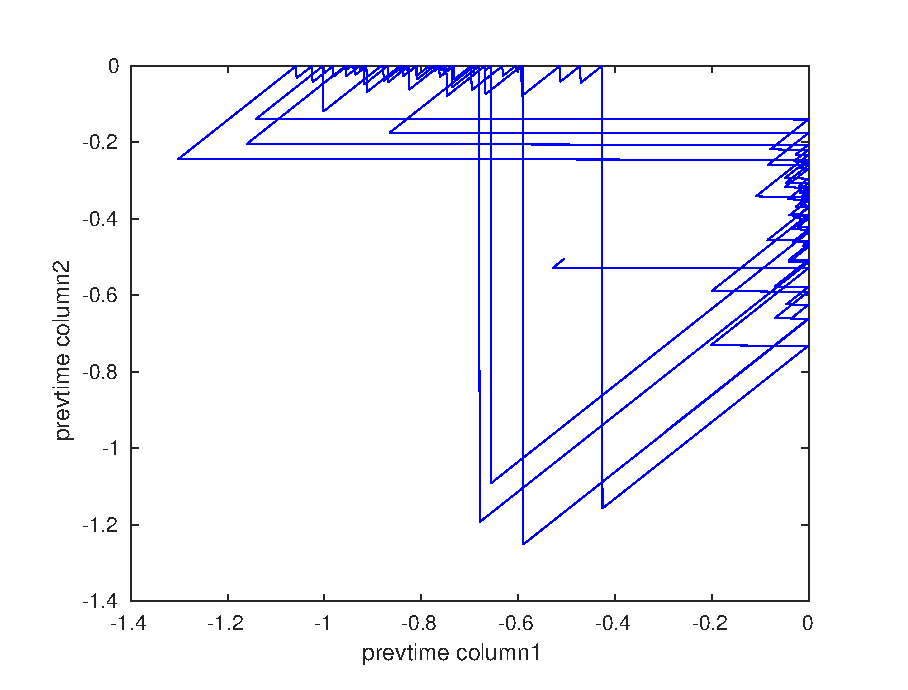
\includegraphics[width=\textwidth]{./images/FinalOralPlots/SyntheticOralPaper/SimPrevtime.eps}
            \caption[]%
            {{\small Simulated previous time data (Prevtime)}}  
            %{{\small Simulated firing rate data (FR)}}    
            \label{fig:Sim animal position in 3D}
        \end{subfigure}
        \vskip\baselineskip
        \begin{subfigure}[b]{0.475\textwidth}   
            \centering 
            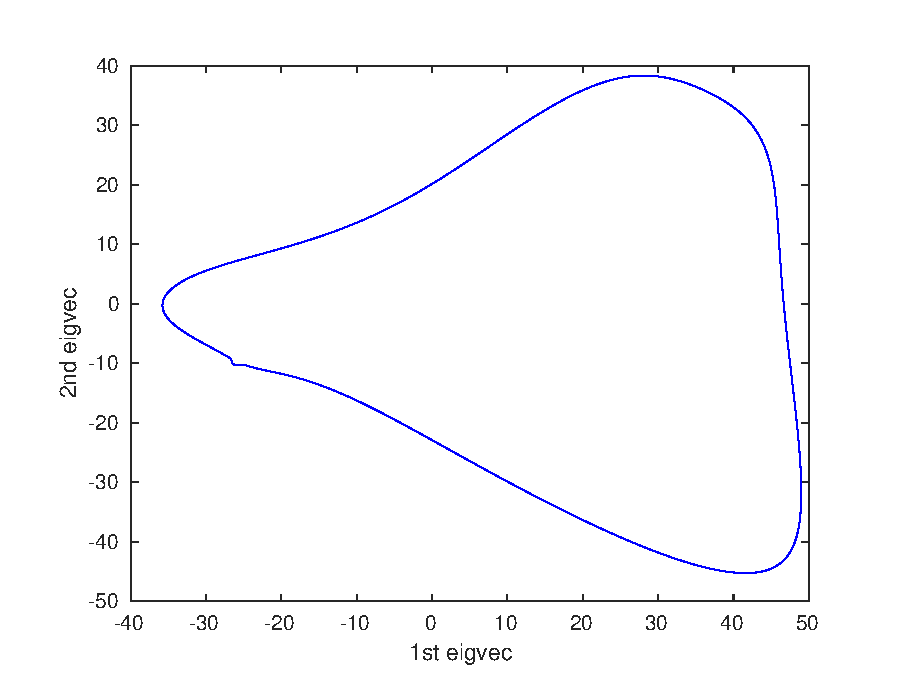
\includegraphics[width=\textwidth]{./images/FinalOralPlots/SyntheticOralPaper/SimFRPCA.eps}
           % 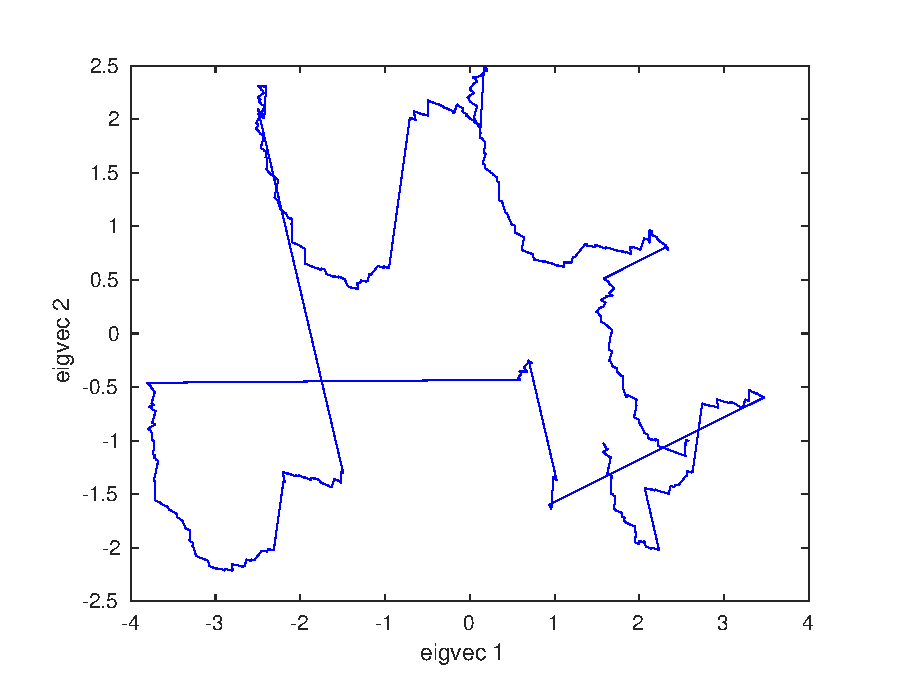
\includegraphics[width=\textwidth]{./images/FinalOralPlots/SyntheticOralPaper/SimPrevtimePCA.eps}
            \caption[]%
             {{\small PCA on FR}}   
            %{{\small PCA on Prevtime}}    
            \label{fig:PCA on Prevtime in 3D}
        \end{subfigure}
        \quad
        \begin{subfigure}[b]{0.475\textwidth}   
            \centering 
            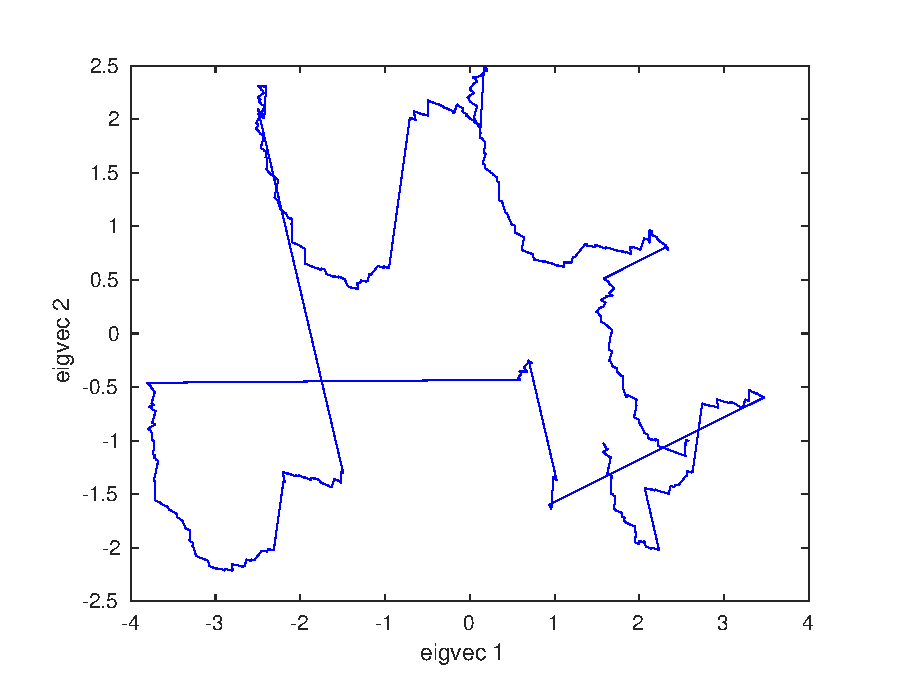
\includegraphics[width=\textwidth]{./images/FinalOralPlots/SyntheticOralPaper/SimPrevtimePCA.eps}
           % 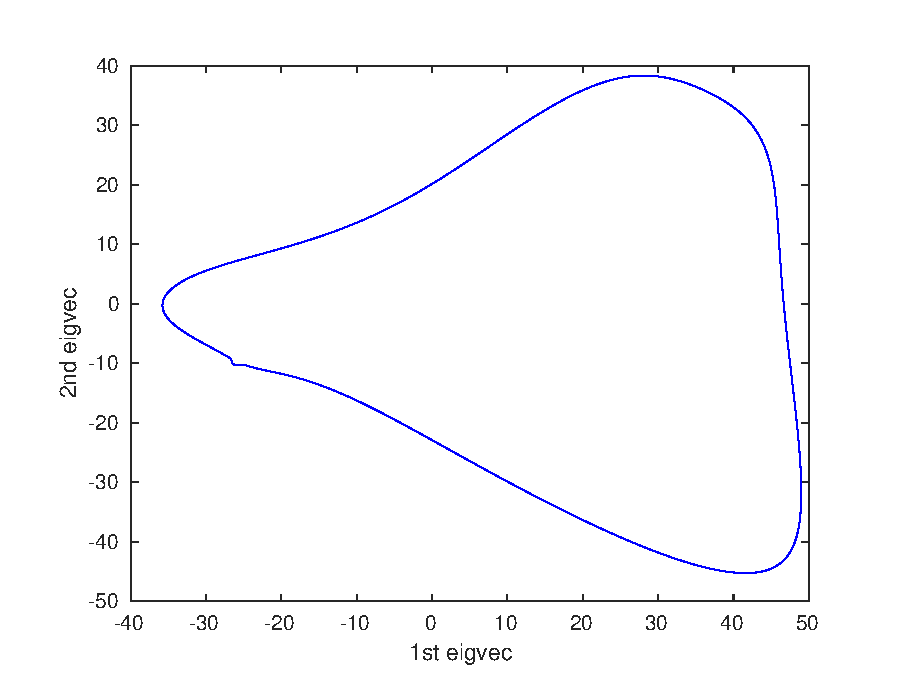
\includegraphics[width=\textwidth]{./images/FinalOralPlots/SyntheticOralPaper/SimFRPCA.eps}
            \caption[]%
             {{\small PCA on Prevtime}}   
           % {{\small PCA on FR}}    
            \label{fig:PCA on prevtime in 2D }
        \end{subfigure}
        \vskip\baselineskip
        \begin{subfigure}[b]{0.475\textwidth}   
            \centering 
             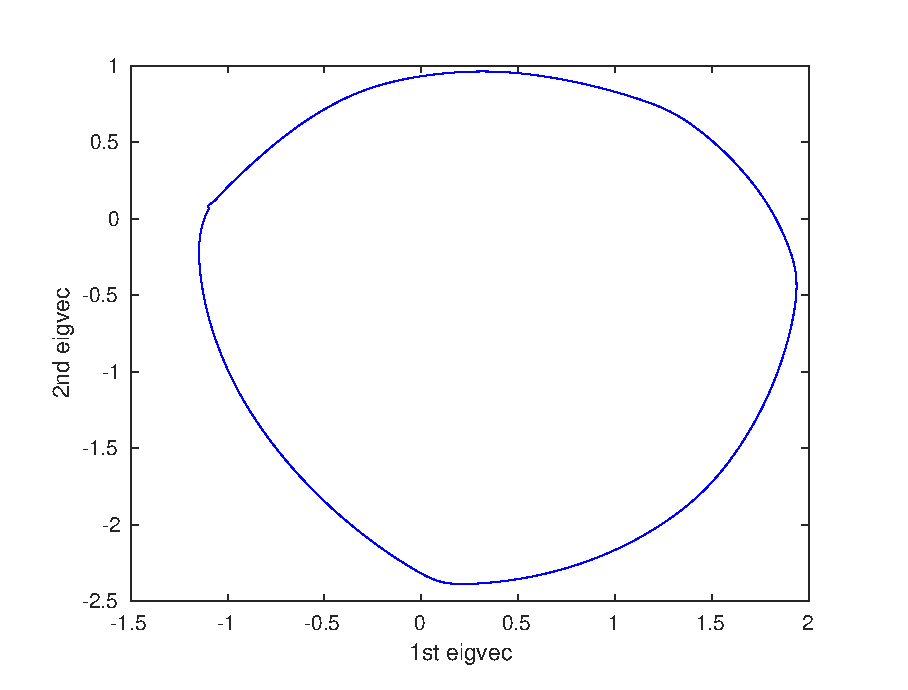
\includegraphics[width=\textwidth]{./images/FinalOralPlots/SyntheticOralPaper/SimFRDML1.eps}
          %  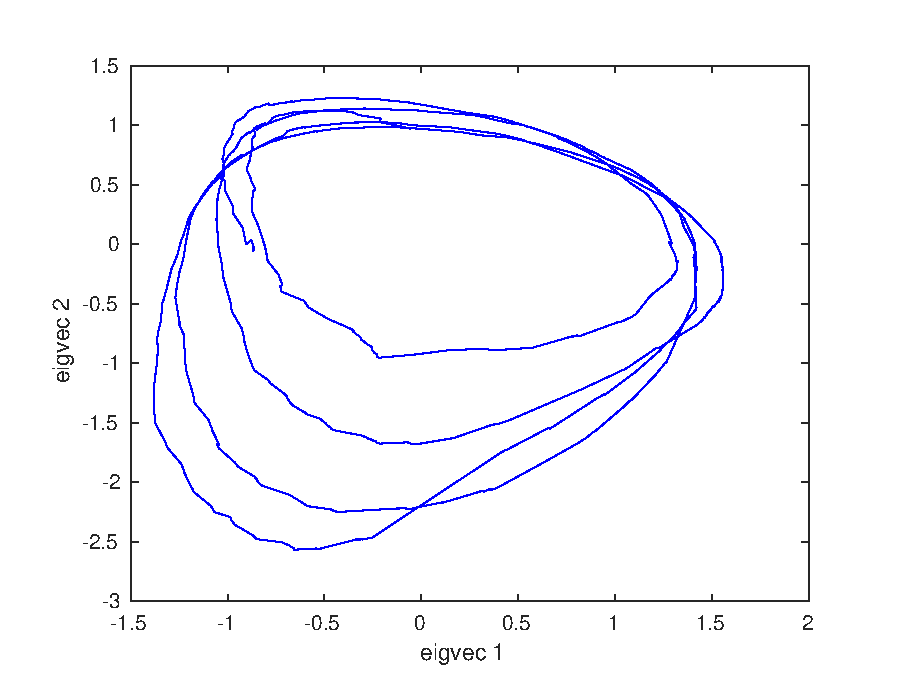
\includegraphics[width=\textwidth]{./images/FinalOralPlots/SyntheticOralPaper/SimPrevtimeDML1.eps}
            \caption[]%
             {{\small Diffusion Maps on FR}}    
            %{{\small Diffusion Maps on Prevtime}}    
            \label{fig:Diffusion maps on Prevtime in 3D}
        \end{subfigure}
        \quad
        \begin{subfigure}[b]{0.475\textwidth}   
            \centering 
             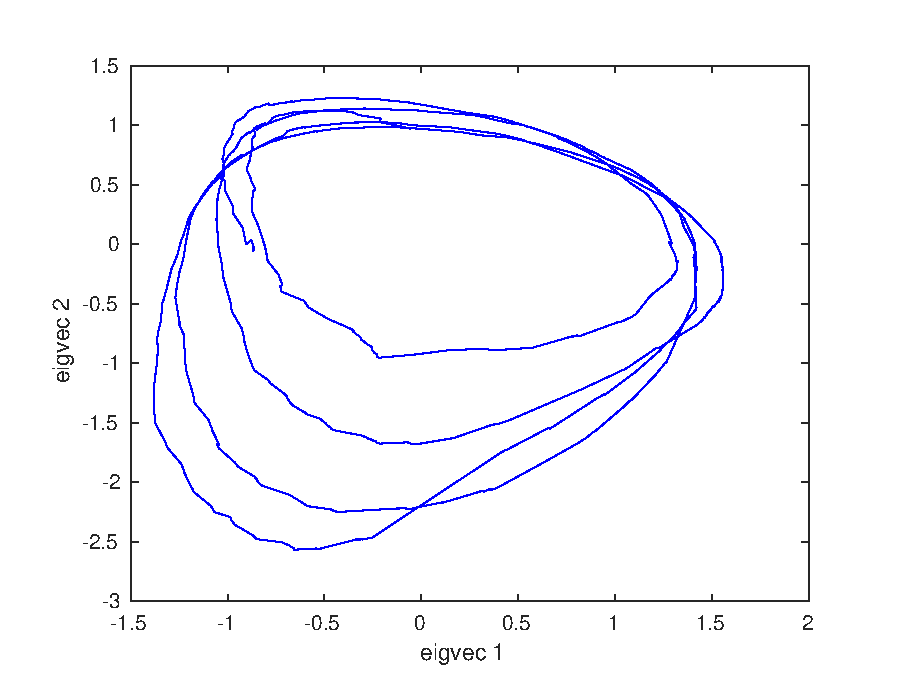
\includegraphics[width=\textwidth]{./images/FinalOralPlots/SyntheticOralPaper/SimPrevtimeDML1.eps}
           % 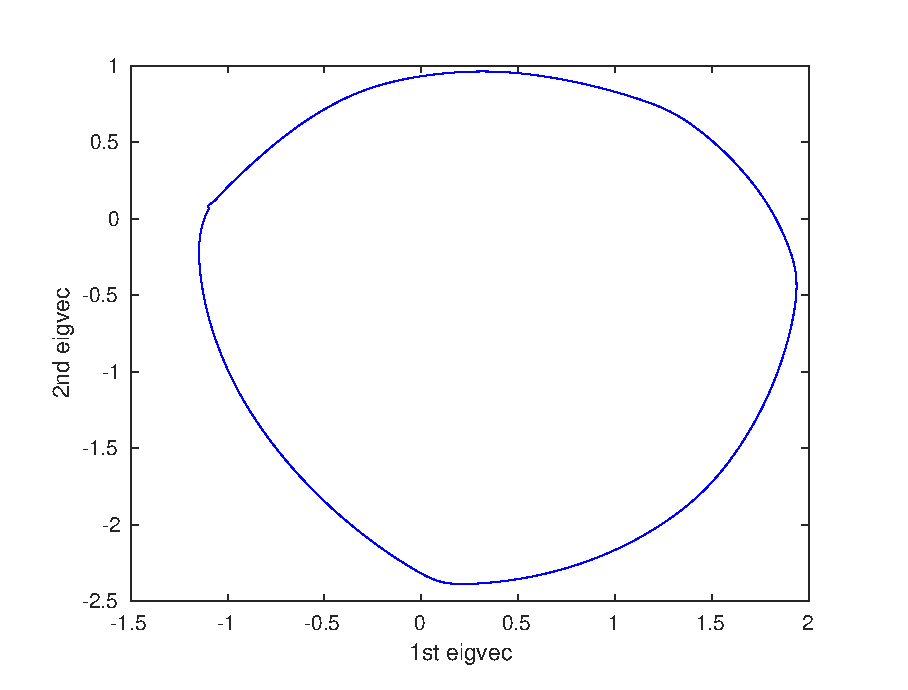
\includegraphics[width=\textwidth]{./images/FinalOralPlots/SyntheticOralPaper/SimFRDML1.eps}
            \caption[]%
            {{\small Diffusion Maps on Prevtime}}  
           % {{\small Diffusion Maps on FR}}    
            \label{fig:Diffusion maps on Prevtime in 3D }
        \end{subfigure}
        \caption[Performance of Diffusion maps and PCA on data ]
         {\small Performance of Diffusion maps (e and f) and PCA (c and d) on simulated firing rate data (a) and on simulated previous  time data (b). The $x$ and $y$ axes in both (a) and (b)  represent the first and second neuron respectively.
         Any single point on a curve  (in c, d, e and f) represents the value of the first eigen vector (x-axis) and
         the second eigen vector (y-axis) at any time $t$. Since the rat's position in space is a circular curve parametrized in time $t$, the top two eigen vectors of diffusion maps on previous time data capture this circular motion as shown in (f).} 
        \label{fig:DiffMaps_PCA_on_Prevtime_FR}
\end{figure}



















%\newpage

%%%%%%%%%%%%%%%%%%%%  Firing rate %%%%%%%%%%%%%%%%%%%%%%%%%%%%%%%%%%%%%%%%%%%%%%%%%%


%\begin{figure}[H]
%        \centering
%        \begin{subfigure}[b]{0.475\textwidth}
%            \centering
%            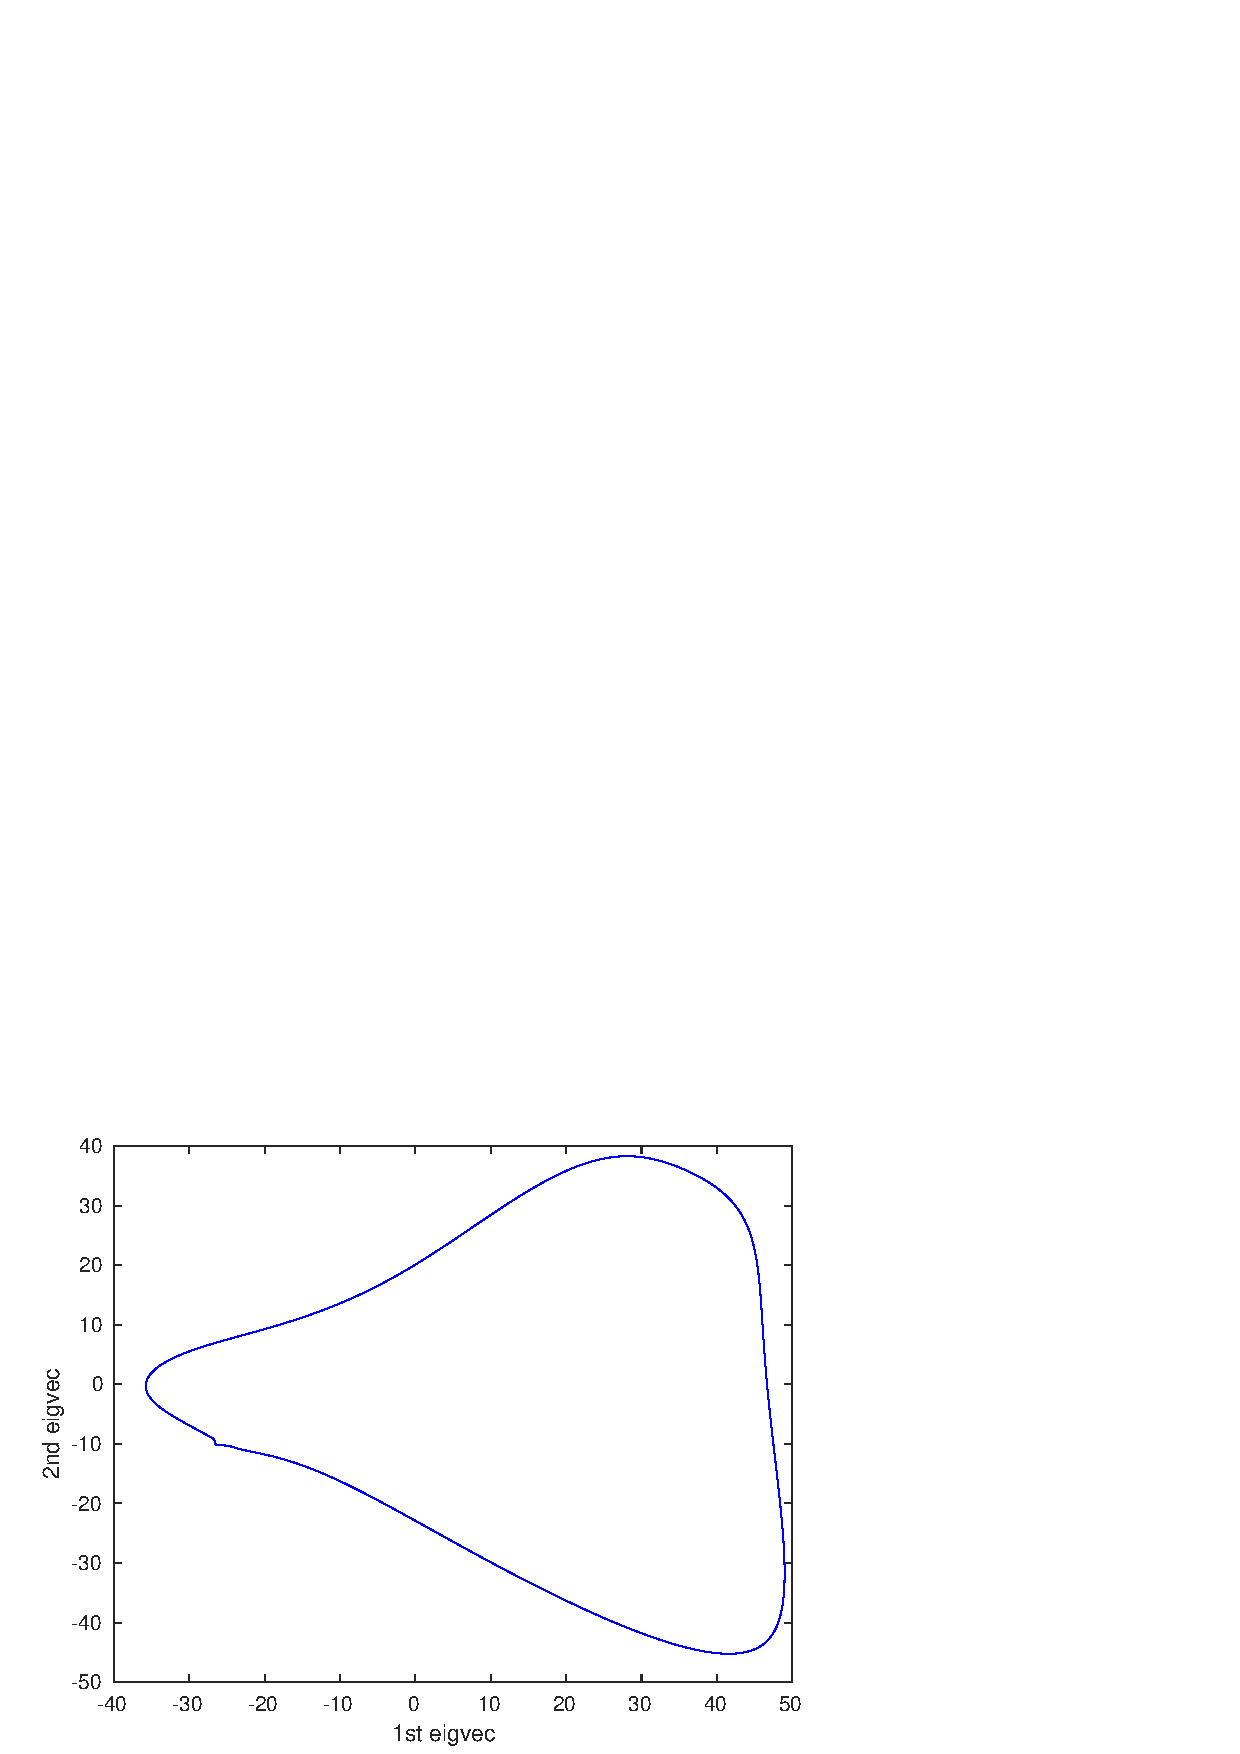
\includegraphics[width=\textwidth]{./images/FinalOralPlots/SyntheticOralPaper/SimFRPCA.pdf}
%            \caption[PCA on FR]%
%            {{\small PCA on FR}}    
%            \label{fig:PCA on FR in 3D}
%        \end{subfigure}
%        \hfill
%        \begin{subfigure}[b]{0.475\textwidth}  
%            \centering 
%            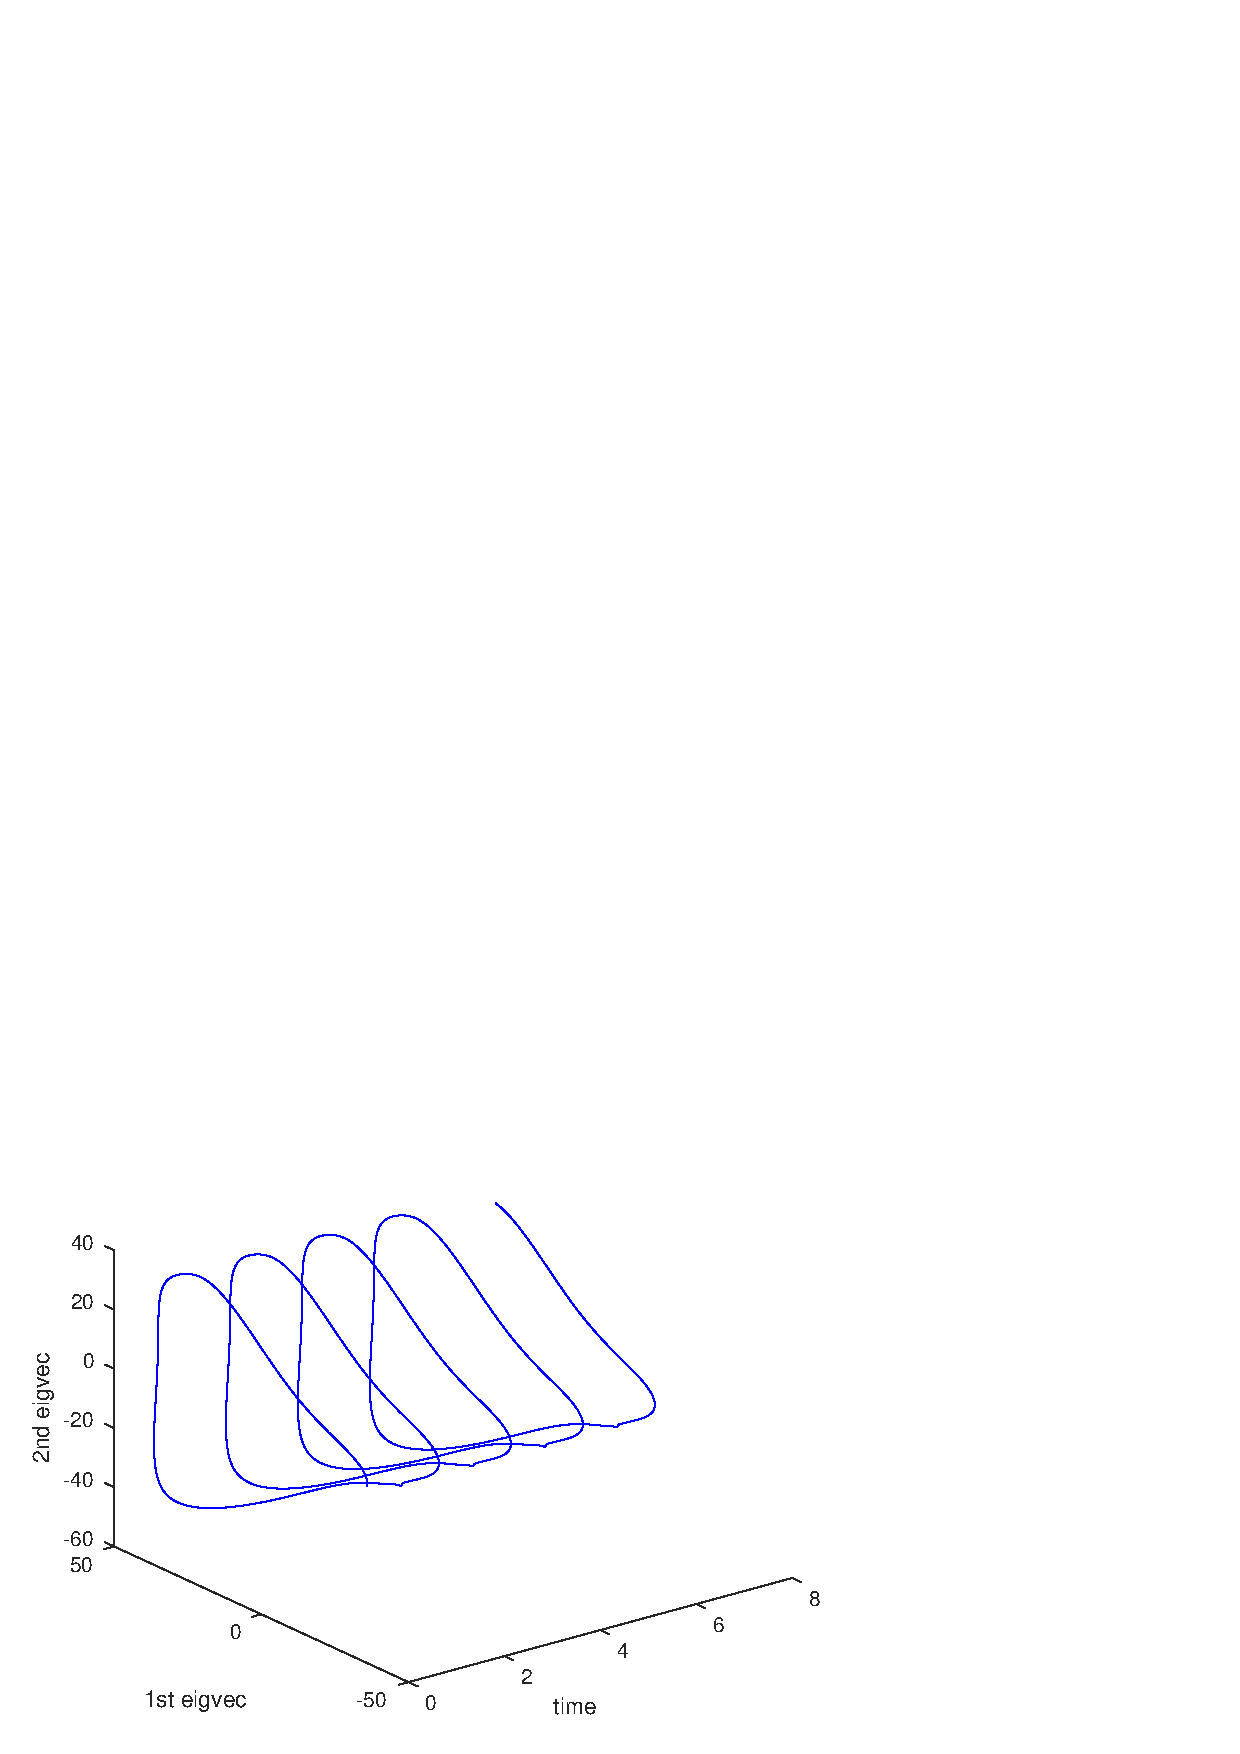
\includegraphics[width=\textwidth]{./images/FinalOralPlots/SyntheticOralPaper/SimFRPCA-with-time.pdf}
%            \caption[]%
%            {{\small PCA on FR}}    
%            \label{fig:PCA on FR in 2D}
%        \end{subfigure}
%        \vskip\baselineskip
%        \begin{subfigure}[b]{0.475\textwidth}   
%            \centering 
%            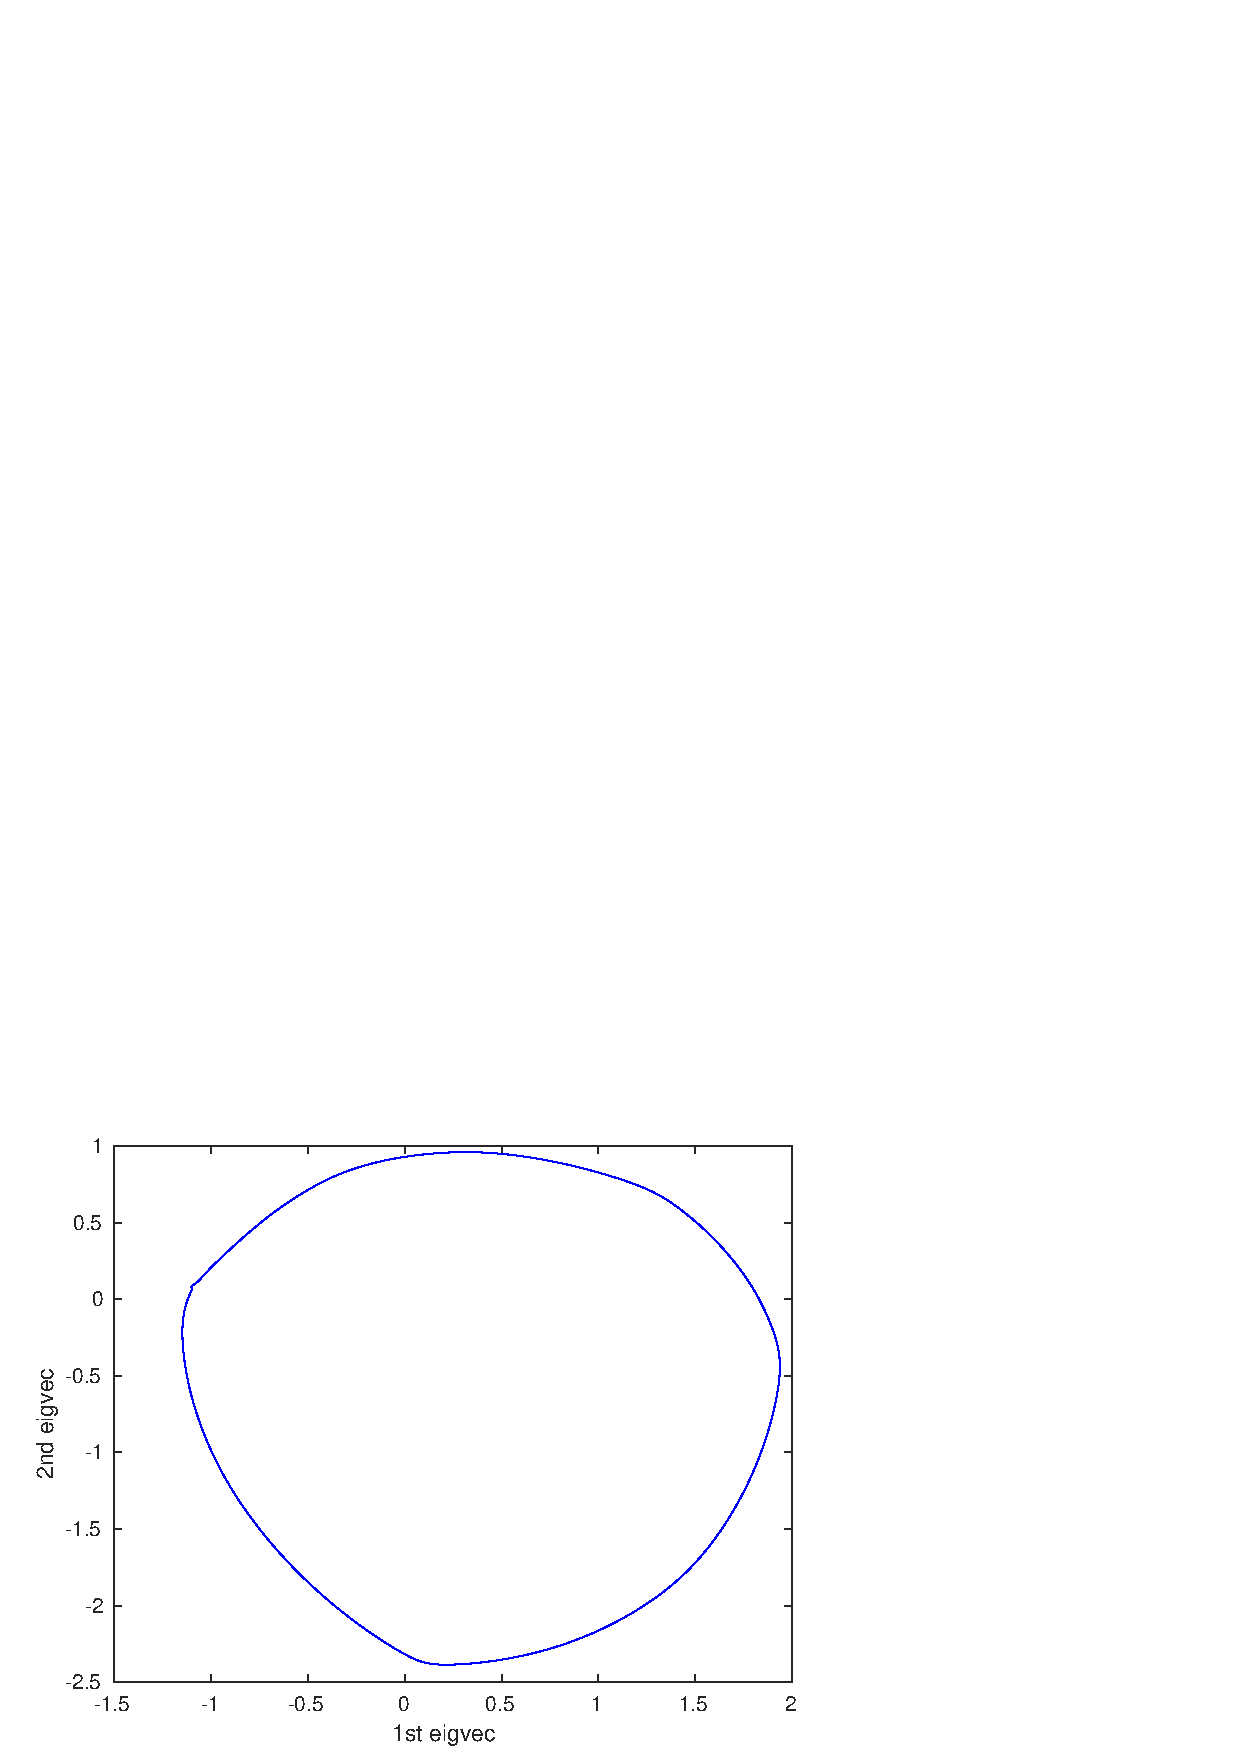
\includegraphics[width=\textwidth]{./images/FinalOralPlots/SyntheticOralPaper/SimFRDML1.pdf}
%            \caption[]%
%            {{\small Diffusion Maps on FR}}    
%            \label{fig:Diffusion maps on FR in 3D}
%        \end{subfigure}
%        \quad
%        \begin{subfigure}[b]{0.475\textwidth}   
%            \centering 
%            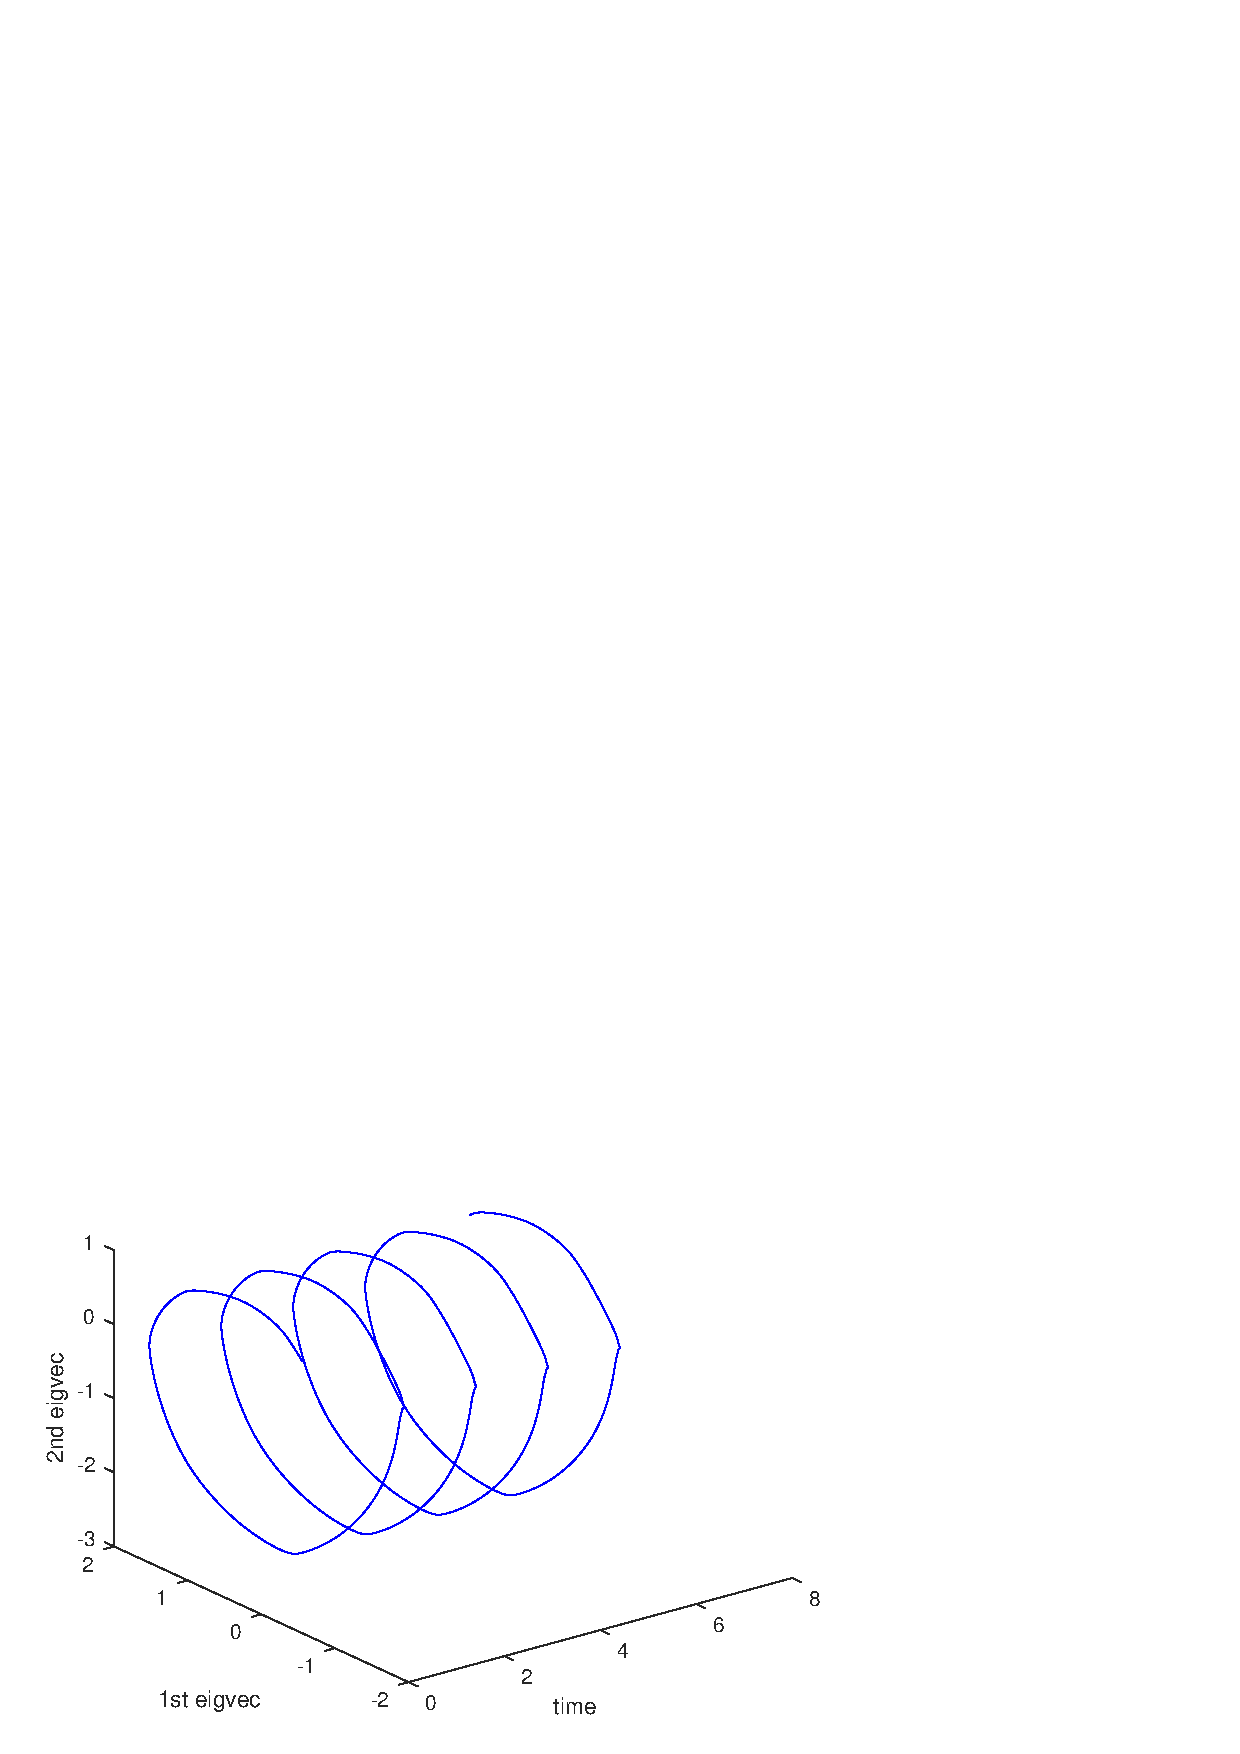
\includegraphics[width=\textwidth]{./images/FinalOralPlots/SyntheticOralPaper/SimFRDML1-with-time.pdf}
%            \caption[]%
%            {{\small Diffusion Maps on FR}}    
%            \label{fig:Diffusion maps on FR in 2D }
%        \end{subfigure}
%        \caption[small Performance of Diffusion maps and PCA on simulated firing rate data ]
%        {\small Performance of Diffusion maps and PCA on simulated firing rate data} 
%        \label{fig:DiffMaps_PCA_on_FR}
%    \end{figure}
%
%


%Next, we show the results of diffusion maps with $l_{1}$ distance 
%and PCA on simulated previous time data (Prevtime). 

%%%%%%%%%%%%%%%%%%%%%%%%%%%% Prevtime and simulated position %%%%%%%%%%%%%%%%%%%%%%%%%%%%%

%\begin{figure}[H]
%        \centering
%        \begin{subfigure}[b]{0.475\textwidth}
%            \centering
%            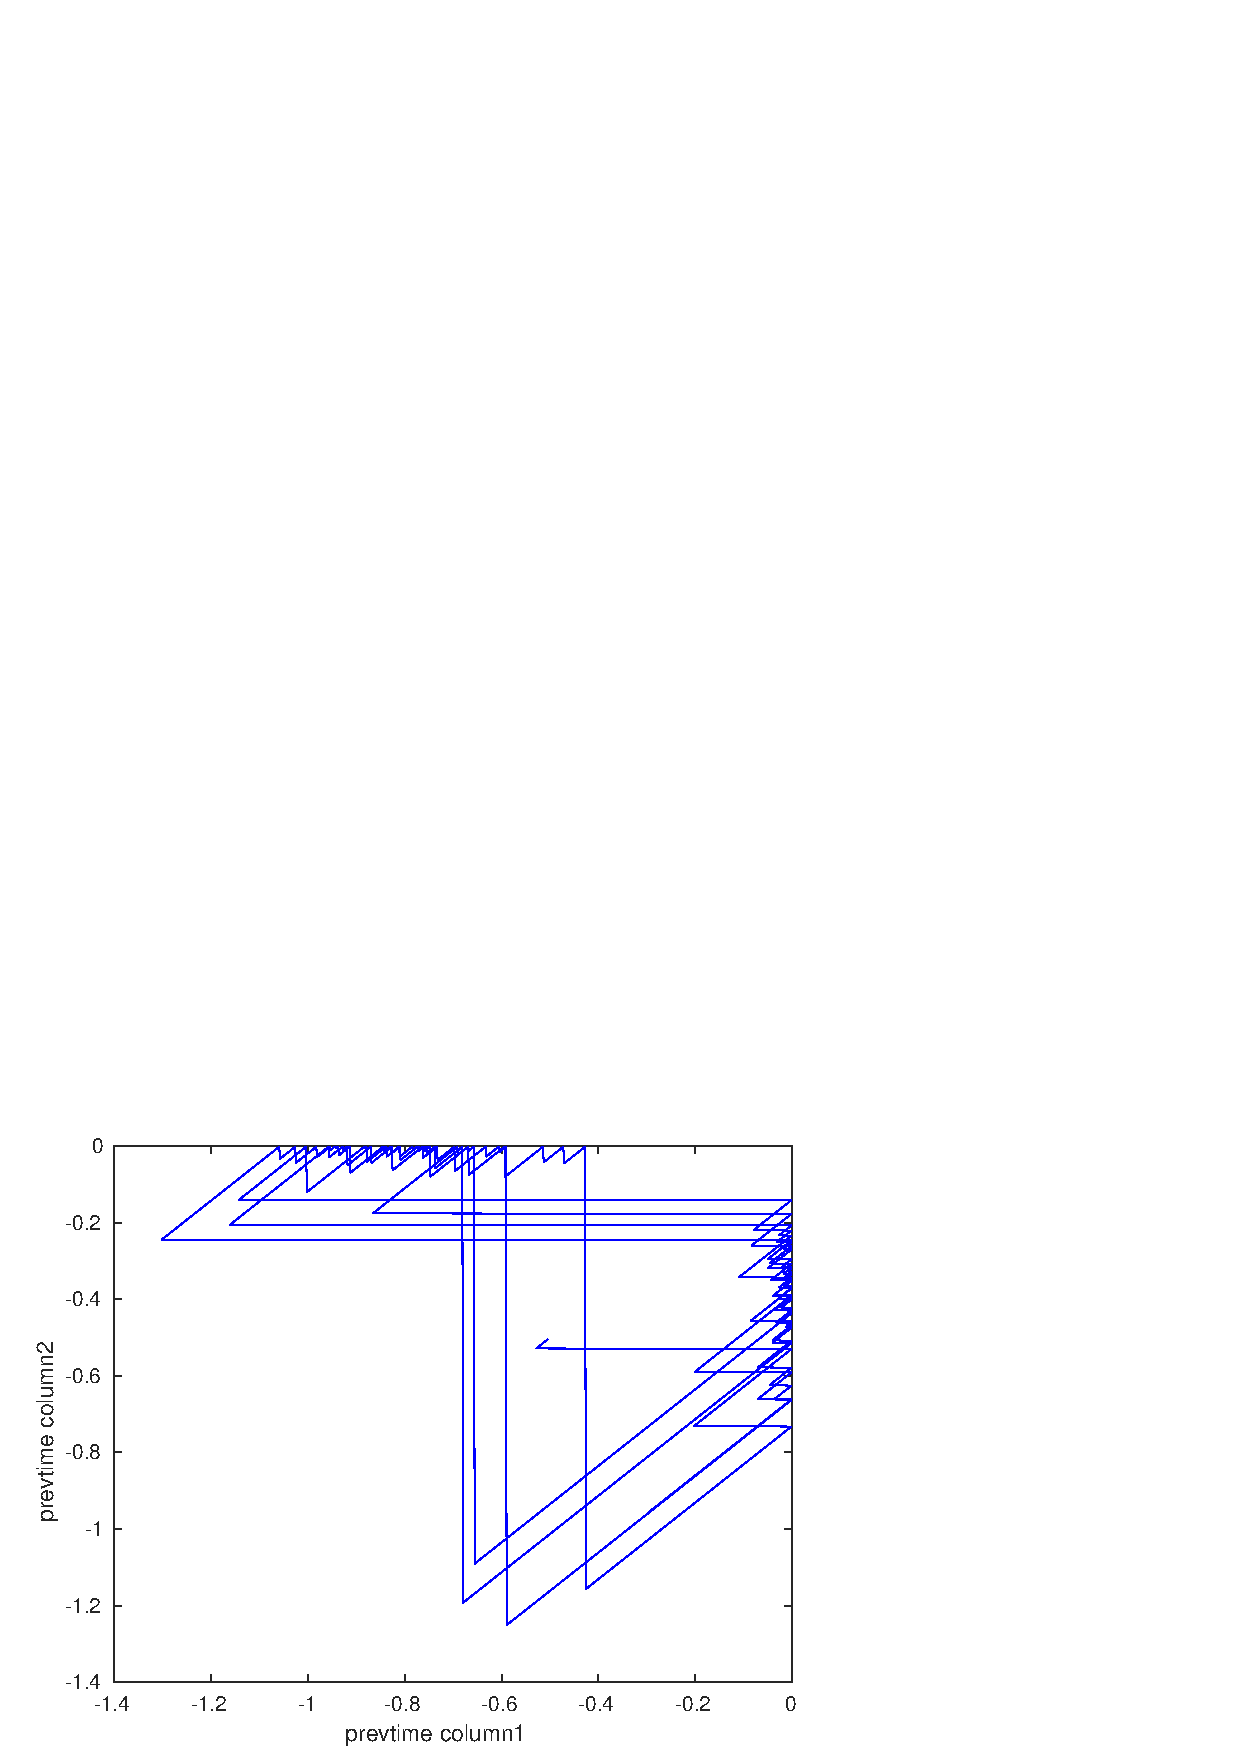
\includegraphics[width=\textwidth]{./images/FinalOralPlots/SyntheticOralPaper/SimPrevtime.pdf}
%            \caption[Simulated Prevtime]%
%            {{\small Simulated Prevtime}}    
%            \label{fig:Prevtime in 3D}
%        \end{subfigure}
%        \hfill
%        \begin{subfigure}[b]{0.475\textwidth}  
%            \centering 
%            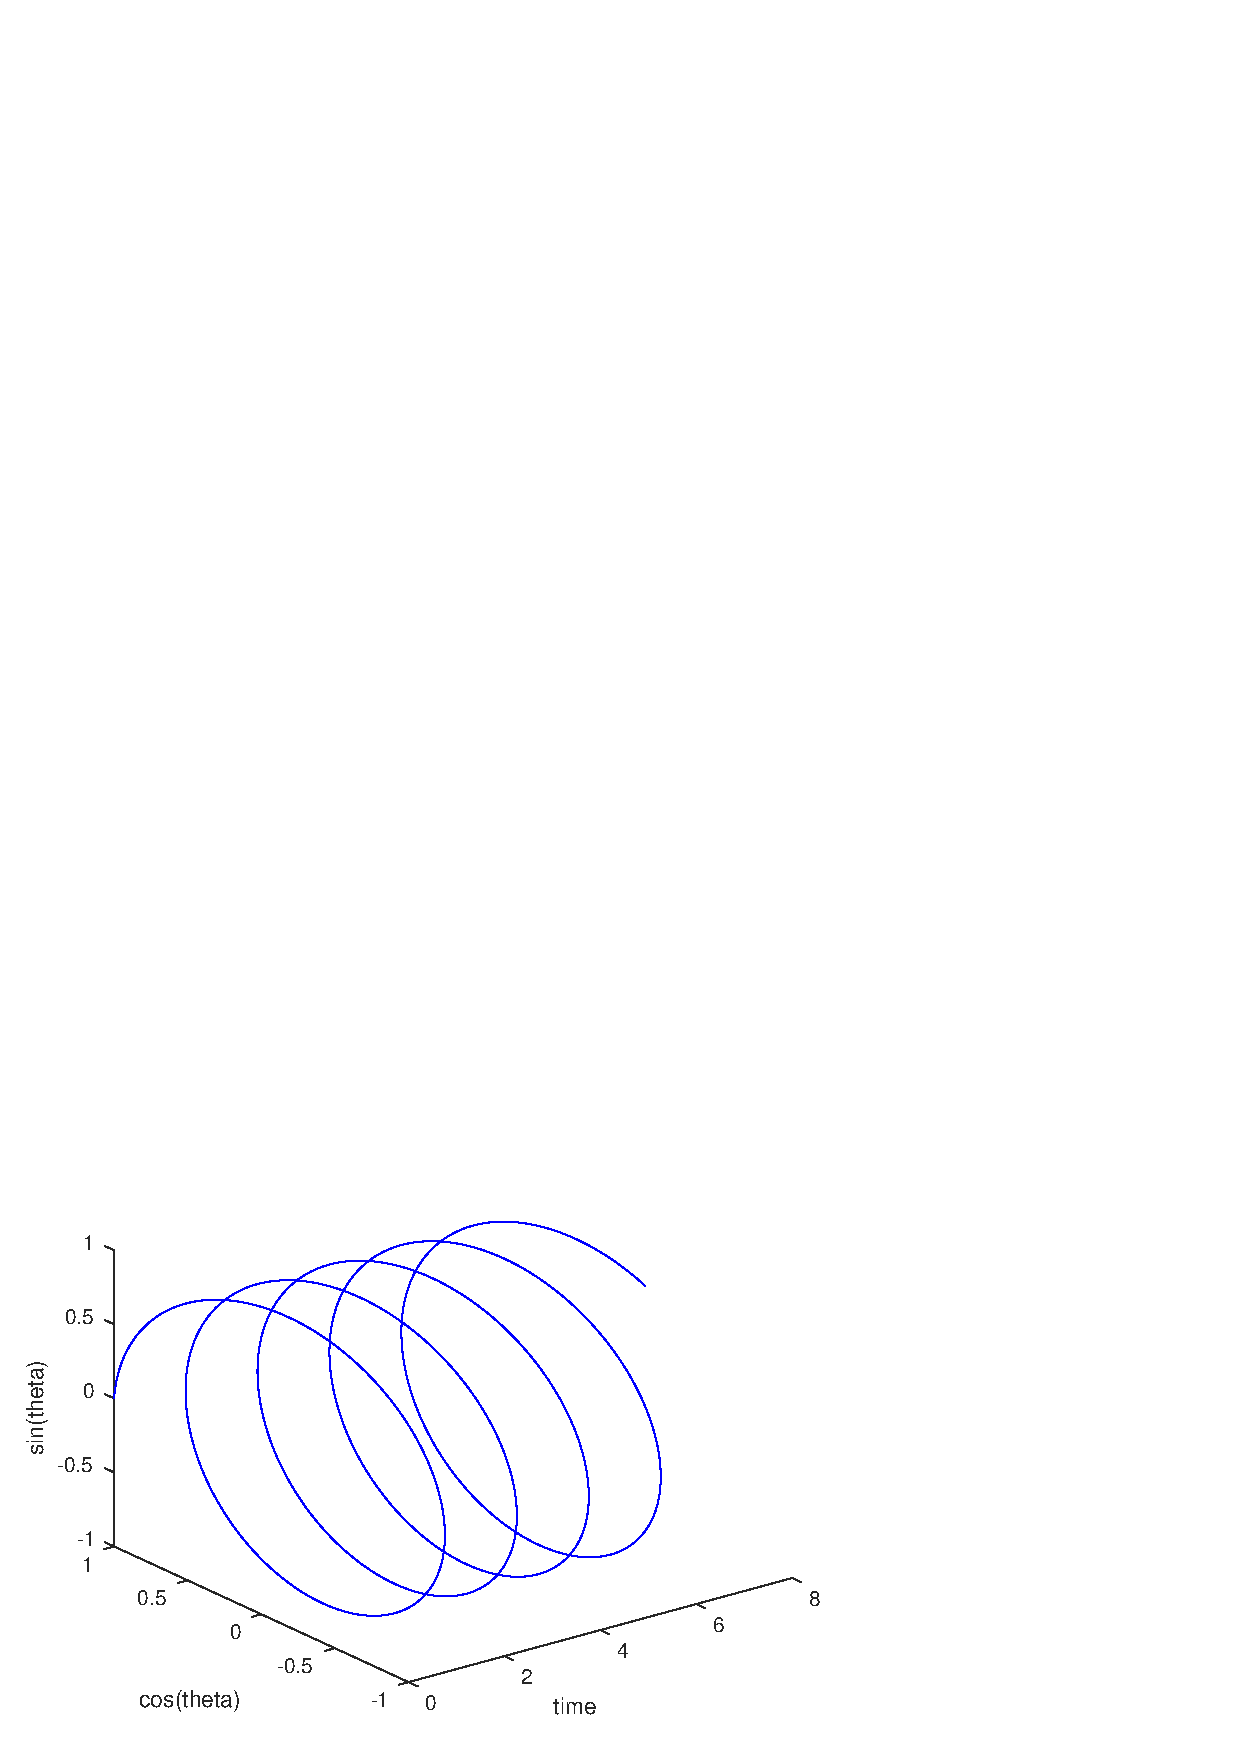
\includegraphics[width=\textwidth]{./images/FinalOralPlots/SyntheticOralPaper/SimRatPosition.pdf}
%            \caption[]%
%            {{\small Simulated animal position}}    
%            \label{fig:Sim animal position in 3D}
%        \end{subfigure}
%        \vskip\baselineskip
%        \begin{subfigure}[b]{0.475\textwidth}   
%            \centering 
%            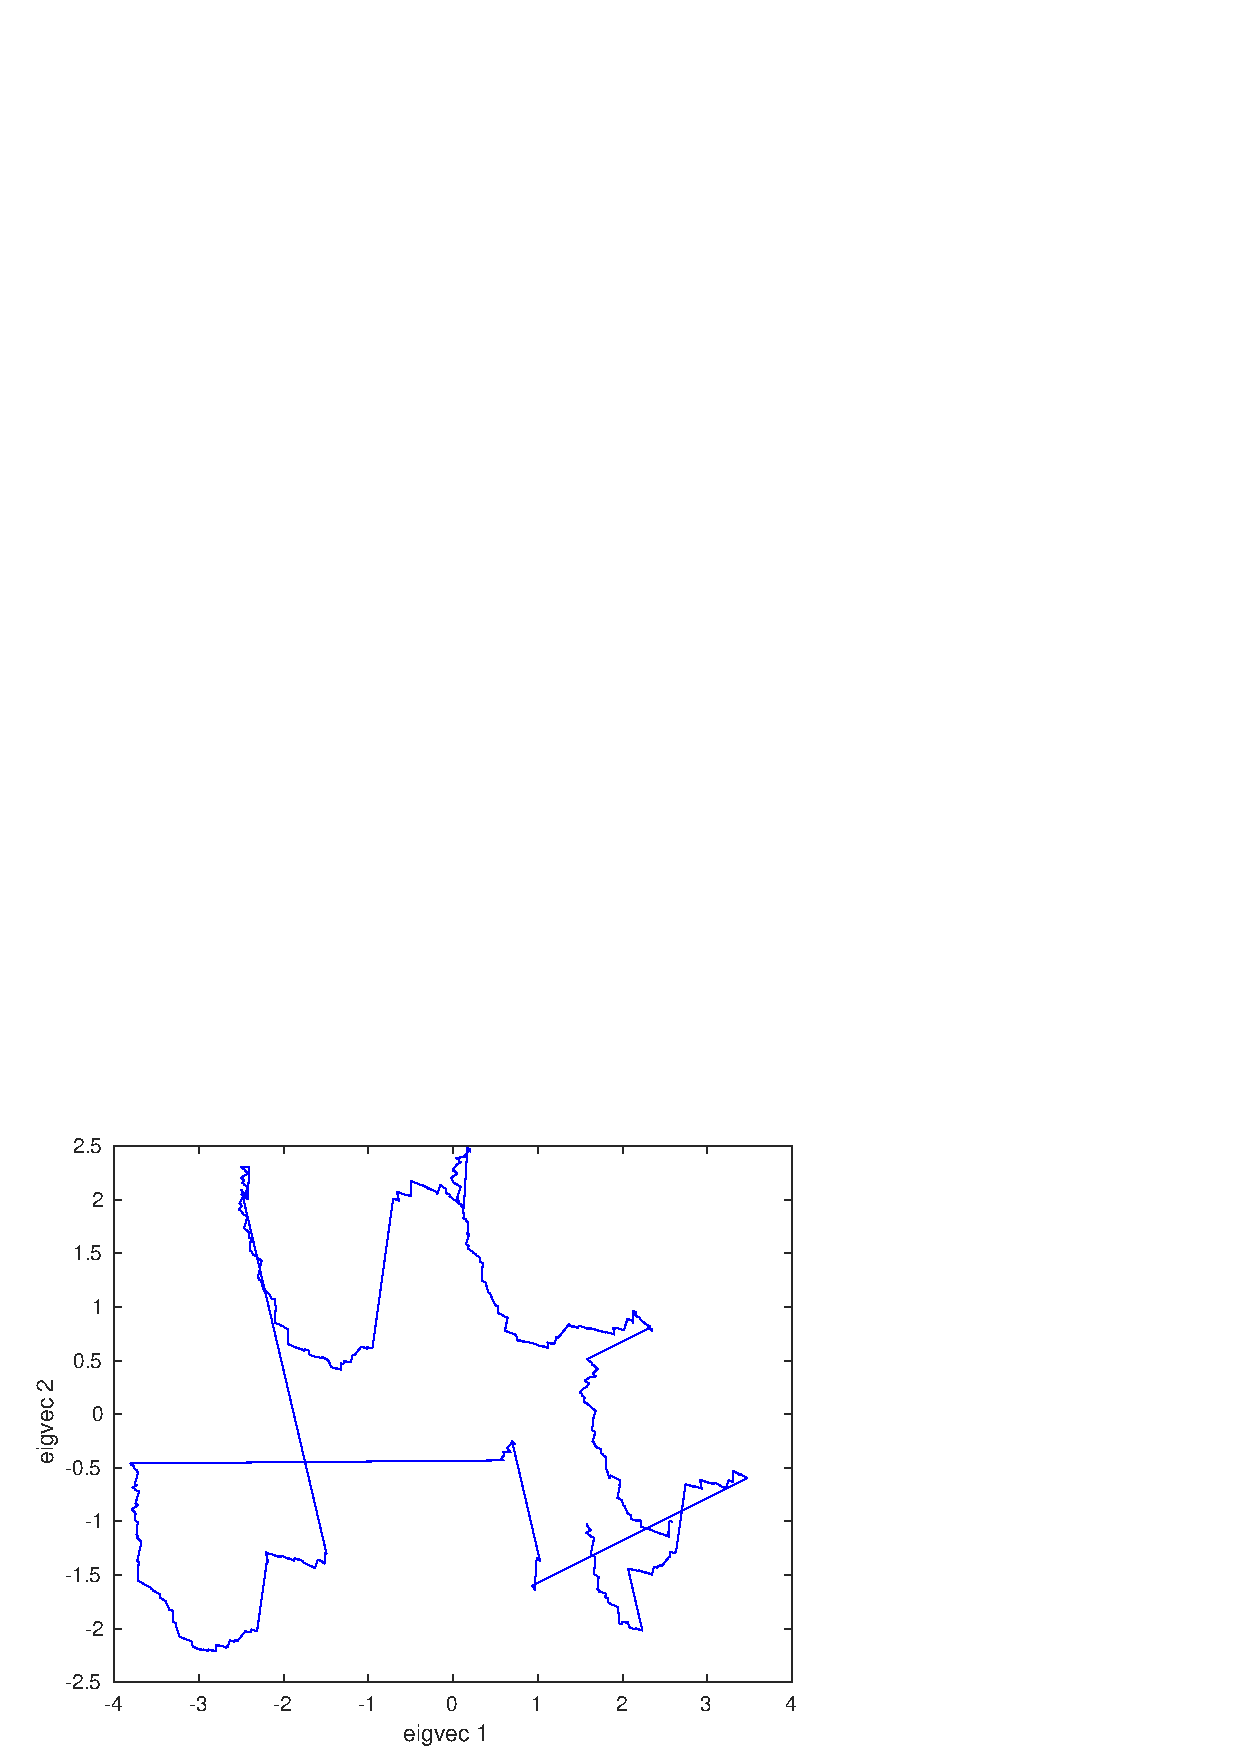
\includegraphics[width=\textwidth]{./images/FinalOralPlots/SyntheticOralPaper/SimPrevtimePCA.pdf}
%            \caption[]%
%            {{\small PCA on Prevtime}}    
%            \label{fig:PCA on Prevtime in 3D}
%        \end{subfigure}
%        \quad
%        \begin{subfigure}[b]{0.475\textwidth}   
%            \centering 
%            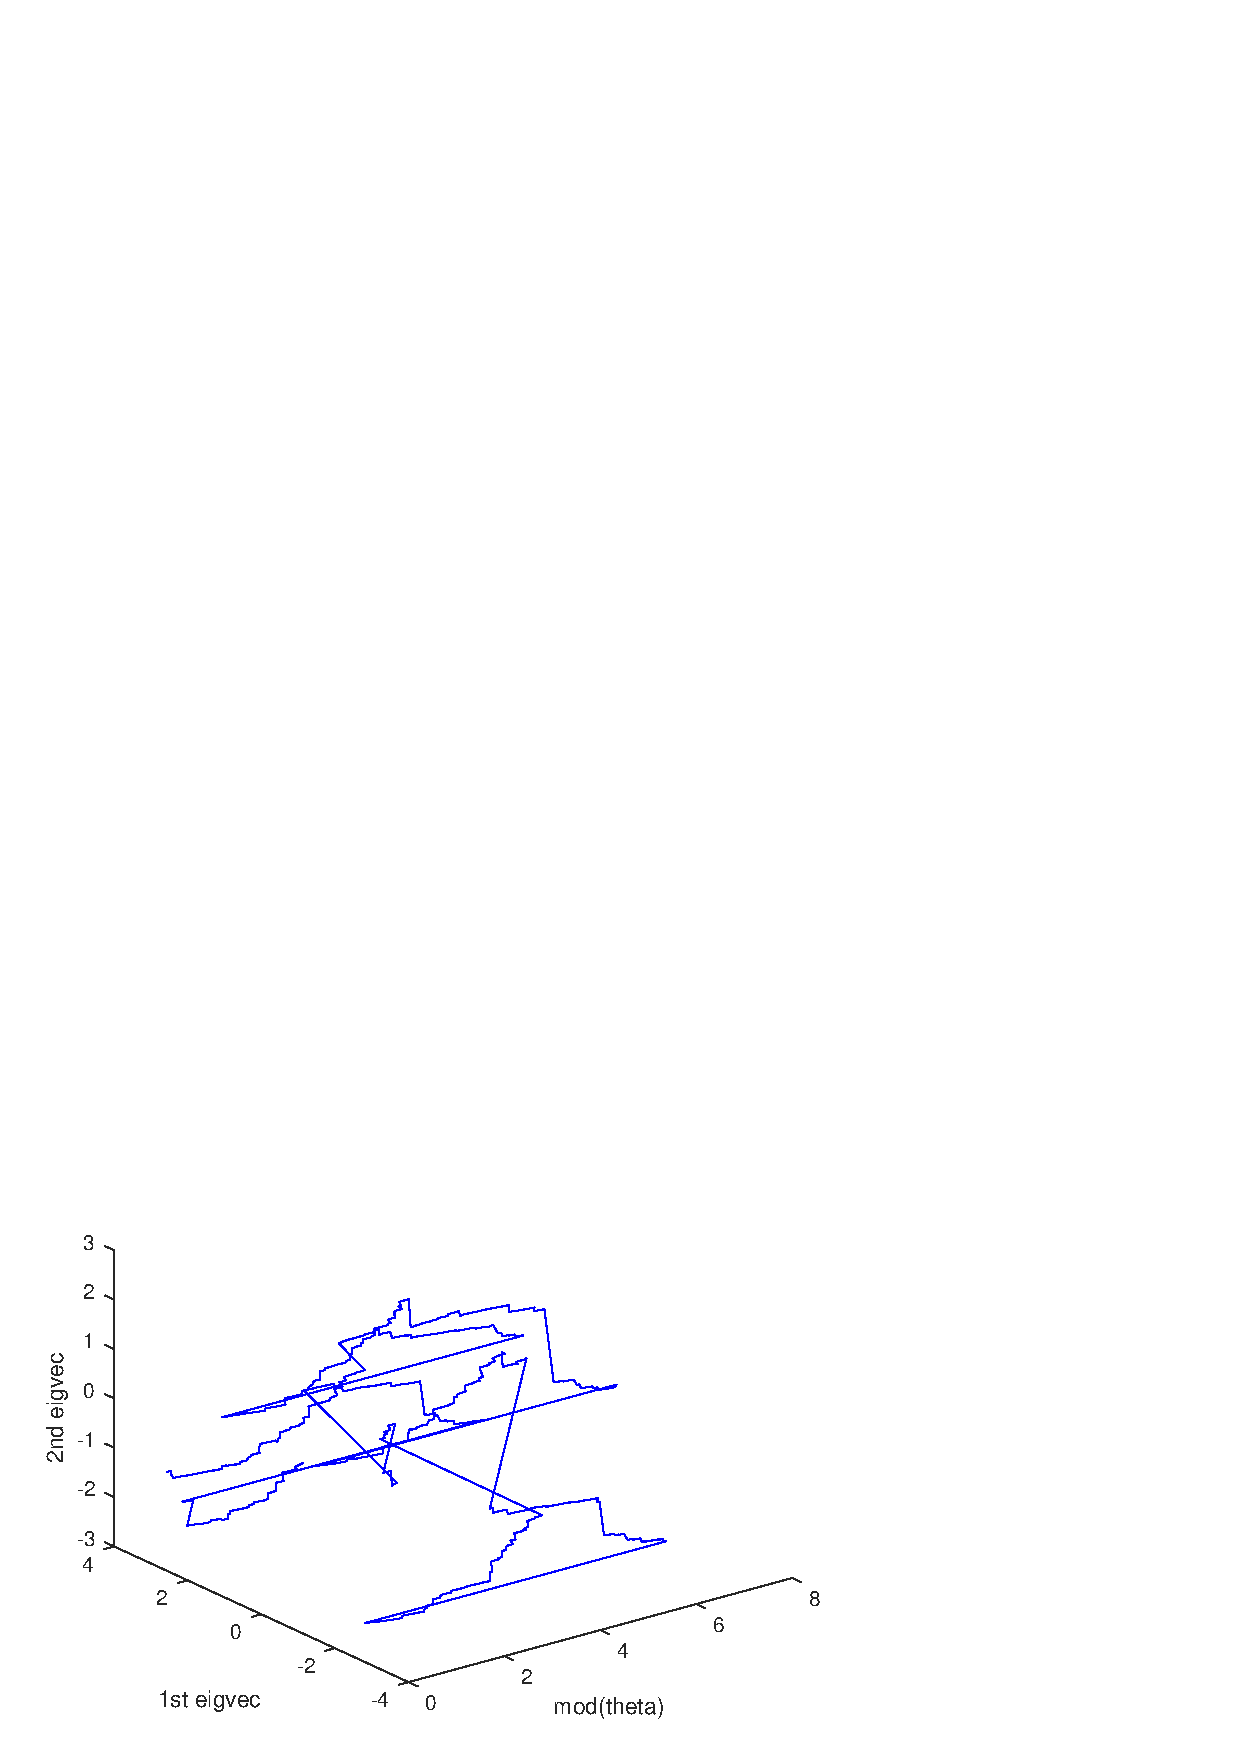
\includegraphics[width=\textwidth]{./images/FinalOralPlots/SyntheticOralPaper/SimPrevtimePCA-with-Position.pdf}
%            \caption[]%
%            {{\small PCA on prevtime}}    
%            \label{fig:PCA on prevtime in 2D }
%        \end{subfigure}
%        \vskip\baselineskip
%        \begin{subfigure}[b]{0.475\textwidth}   
%            \centering 
%            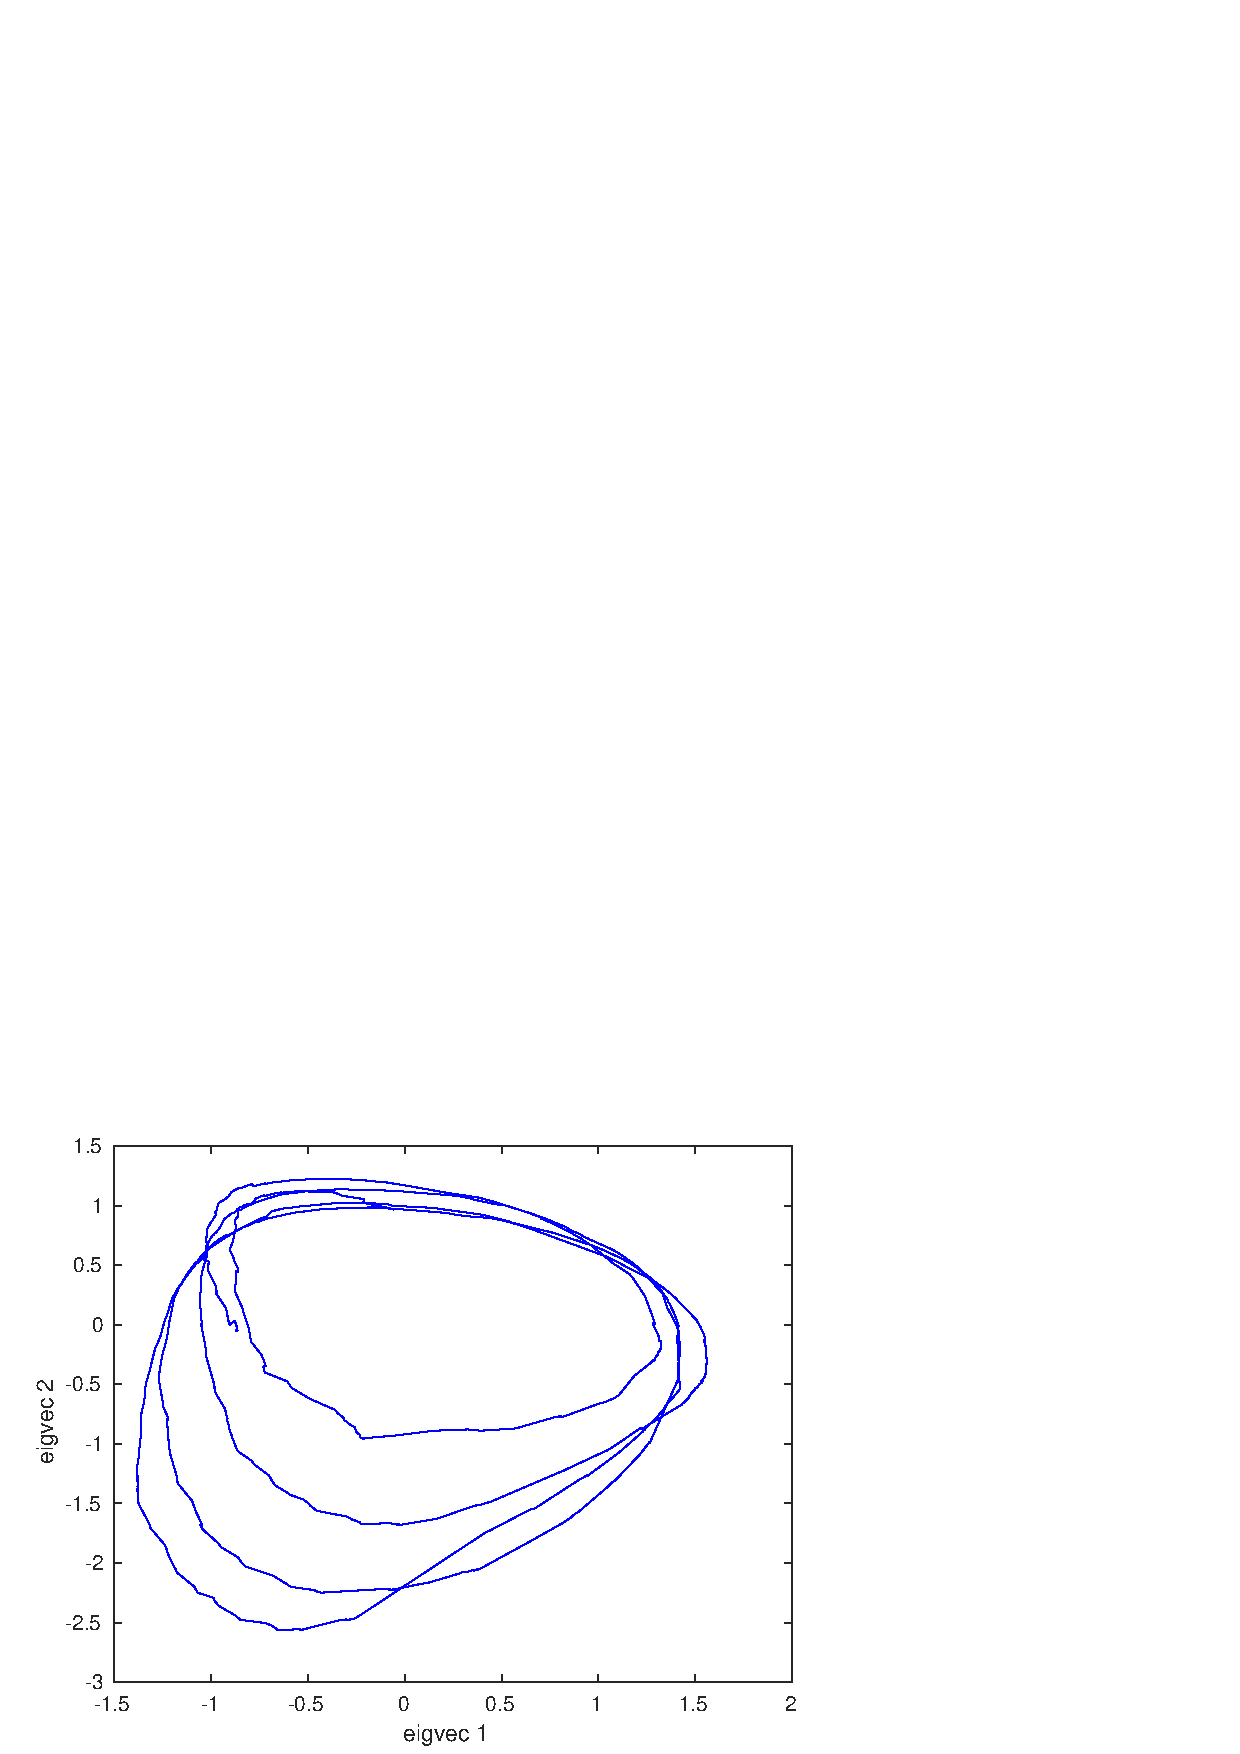
\includegraphics[width=\textwidth]{./images/FinalOralPlots/SyntheticOralPaper/SimPrevtimeDML1.pdf}
%            \caption[]%
%            {{\small Diffusion Maps on Prevtime}}    
%            \label{fig:Diffusion maps on Prevtime in 3D}
%        \end{subfigure}
%        \quad
%        \begin{subfigure}[b]{0.475\textwidth}   
%            \centering 
%            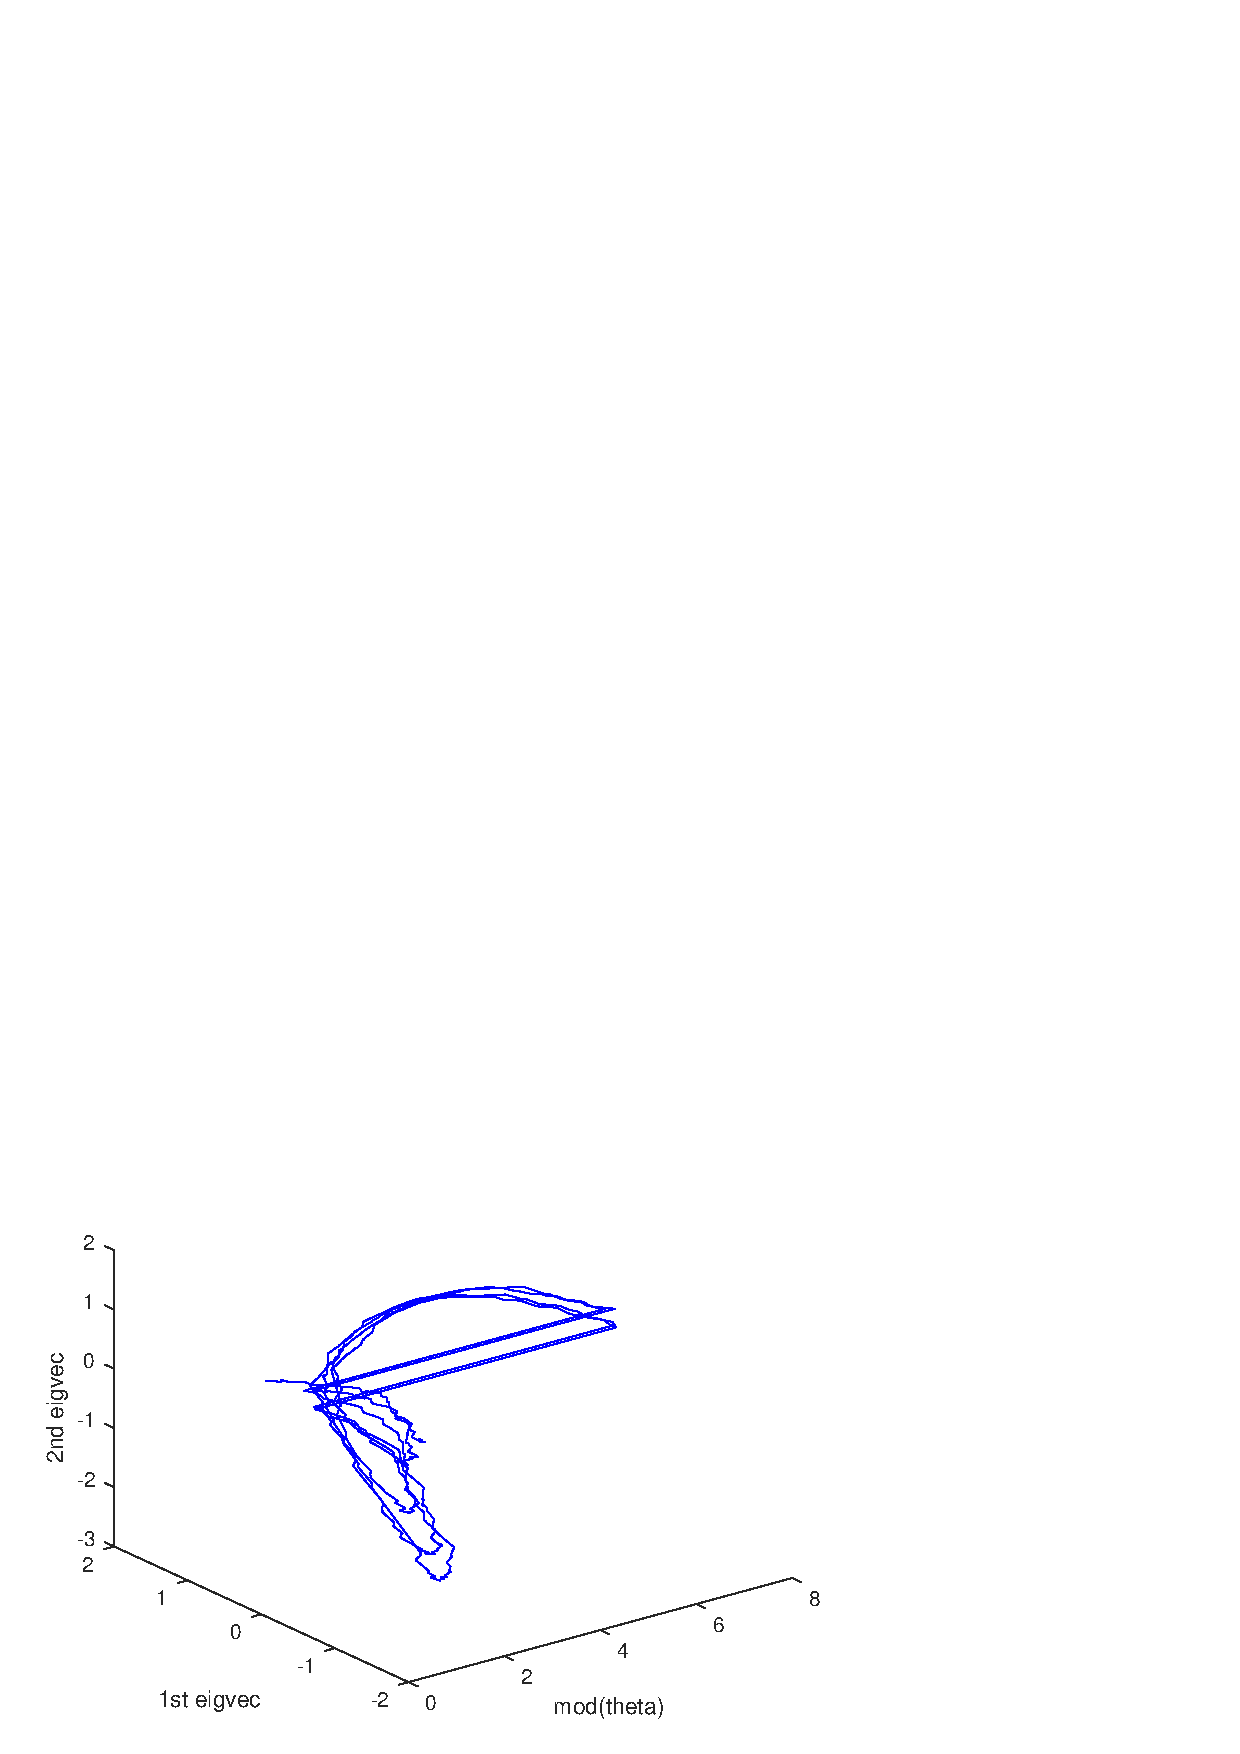
\includegraphics[width=\textwidth]{./images/FinalOralPlots/SyntheticOralPaper/SimPrevtimeDML1-with-Position.pdf}
%            \caption[]%
%            {{\small Diffusion Maps on Prevtime}}    
%            \label{fig:Diffusion maps on Prevtime in 3D }
%        \end{subfigure}
%        \caption[Performance of Diffusion maps and PCA on simulated previous time data ]
%        {\small Performance of Diffusion maps and PCA on simulated previous time data} 
%        \label{fig:DiffMaps_PCA_on_Prevtime}
%\end{figure}
%


















 































































%\begin{itemize}
%\item show the graphs/results package
%\item this is how we're interpreting the results
%\item why does this matter?
%\item what measure of goodness did you use?
%(Fisher Vs Shannon information)

%%==========suggested by Duane============================================
%\item Mention that there are other ways of checking measures of goodness
% e.g the one provided by diffusion maps, Bayesian decoding refer to the nature
% and review artcicle.


%\end{itemize}







